\chapter{Desarrollo}
\label{ch.ej5:desarrollo}

En esta sección se analiza detalladamente el diseño del firmware, la configuración de los periféricos involucrados,
los cálculos teóricos de frecuencia y ciclo de trabajo (\textit{Duty Cycle}), y el principio físico que relaciona la
modificación del registro de comparación con la intensidad lumínica percibida en el LED.

\section{Descripción del Funcionamiento del Programa}
\label{sec.ej5:funcionamiento}

El programa implementa una estructura cooperativa no bloqueante asistida por dos periféricos de hardware:
\begin{enumerate}
    \item \textbf{Base de Tiempo del Sistema (\textit{SysTick}):} El temporizador \textit{SysTick} se programa para
    generar una interrupción periódica cada $\qty{1}{\ms}$. Dentro del controlador de interrupción
    \lstinline{SysTick_Handler}, se incrementa una variable global volátil \lstinline{ms_ticks}.
    \item \textbf{Generador PWM por Hardware (\texttt{TIM1}):} El temporizador avanzado \texttt{TIM1} genera autónomamente
    una señal PWM de $\qty{1}{\kHz}$ en el pin \texttt{PA8} (\texttt{TIM1\_CH1}). La oscilación y conmutación lógica
    del pin es efectuada directamente por el periférico de hardware, sin intervención del procesador principal.
    \item \textbf{Bucle Principal Concurrente:} En el bucle principal \lstinline{while(1)}, se administran dos tareas
    independientes utilizando las marcas de tiempo obtenidas de \lstinline{ms_ticks}:
    \begin{itemize}
        \item \textbf{Parpadeo Testigo (\texttt{PC13}):} Cada $\qty{200}{\ms}$, conmuta el estado lógico del LED
        integrado en la placa mediante una operación XOR sobre el registro \lstinline{ODR}.
        \item \textbf{Variación de Brillo (\textit{Fading}):} Cada $\qty{10}{\ms}$, actualiza el registro de comparación
        \lstinline{TIM1->CCR1} modificando el valor de la variable \lstinline{brightness} en pasos de 5 unidades dentro
        del intervalo $[0, 1000]$. Esto produce una rampa continua de variación de brillo en el LED conectado a
        \texttt{PA8} con un ciclo total de $\qty{4}{\s}$ ($\qty{2}{\s}$ de incremento y $\qty{2}{\s}$ de decremento).
    \end{itemize}
\end{enumerate}

\section{Configuración de GPIO y Temporizador}
\label{sec.ej5:configuracion}

El esquema de conexión eléctrica del LED exterior al pin \texttt{PA8} se ilustra en la figura~\ref{crkt.ej5:led_circuit}.

\begin{figure}[!ht]
  \centering
  \begin{circuitikz}[line width=0.8pt]
  \draw (0,0) node[left] {\texttt{PA8 (TIM1\_CH1)}}
        to[short, o-*] (1,0)
        to[R, l={$R_{\mathrm{lim}} = \qty{330}{\ohm}$}] (3.5,0)
        to[led, l={LED}] (5,0)
        node[ground] {};
\end{circuitikz}

  \caption{Esquema de conexión del LED exterior al pin \texttt{PA8} de la placa BluePill.}
  \label{crkt.ej5:led_circuit}
\end{figure}

Para la correcta generación de la señal PWM, se configuraron los siguientes periféricos mediante CMSIS:

\subsection{Habilitación de Relojes de Periféricos (\texttt{RCC})}
Se activaron los relojes para los puertos \texttt{GPIOA}, \texttt{GPIOC} y el temporizador \texttt{TIM1} en el bus APB2:
\begin{lstlisting}[language=C]
RCC->APB2ENR |= RCC_APB2ENR_IOPAEN | RCC_APB2ENR_IOPCEN | RCC_APB2ENR_TIM1EN;
\end{lstlisting}

\subsection{Configuración de Puertos GPIO}
\begin{itemize}
    \item \textbf{Pin \texttt{PC13}:} Salida digital push-pull convencional a $\qty{2}{\MHz}$ (\lstinline{MODE13 = 10b},
    \lstinline{CNF13 = 00b}).
    \item \textbf{Pin \texttt{PA8}:} Configurado como \textbf{Función Alternativa Push-Pull} a $\qty{50}{\MHz}$
    (\lstinline{MODE8 = 11b}, \lstinline{CNF8 = 10b}). Esta selección conmuta el control físico de la línea de salida
    hacia el canal del temporizador \texttt{TIM1\_CH1}:
\end{itemize}
\begin{lstlisting}[language=C]
GPIOA->CRH &= ~(GPIO_CRH_MODE8 | GPIO_CRH_CNF8);
GPIOA->CRH |= (3 << GPIO_CRH_MODE8_Pos) | (2 << GPIO_CRH_CNF8_Pos);
\end{lstlisting}

\subsection{Configuración del Temporizador \texttt{TIM1}}
El módulo \texttt{TIM1} se programó ajustando los siguientes registros:
\begin{enumerate}
    \item \textbf{Preescalador (\lstinline{TIM1->PSC = 7}):} Divide la frecuencia del reloj de entrada
    $f_{\mathrm{CK\_PSC}} = \qty{8}{\MHz}$ por $(\text{PSC} + 1) = 8$, obteniendo una frecuencia de conteo de $\qty{1}{\MHz}$.
    \item \textbf{Autorrecarga (\lstinline{TIM1->ARR = 999}):} Determina el límite superior del contador (1000 conteos
    totales, desde 0 hasta 999).
    \item \textbf{Modo de Canal (\lstinline{TIM1->CCMR1}):}
    \begin{itemize}
        \item \lstinline{OC1M[2:0] = 110b}: Define el Canal 1 en \textbf{PWM Modo 1}. La salida permanece en nivel alto
        mientras $\text{CNT} < \text{CCR1}$ y conmuta a nivel bajo cuando $\text{CNT} \ge \text{CCR1}$.
        \item \lstinline{OC1PE = 1}: Habilita la precarga del registro de comparación (\textit{Preload Enable}), evitando
        conmutaciones espurias (\textit{glitches}) durante las modificaciones del ciclo de trabajo.
    \end{itemize}
    \item \textbf{Habilitación de Salida (\lstinline{TIM1->CCER}):} Habilita el Canal 1 (\lstinline{CC1E = 1}) con
    polaridad activa en alto (\lstinline{CC1P = 0}).
    \item \textbf{Habilitación Principal (\lstinline{TIM1->BDTR}):} En temporizadores avanzados es obligatorio activar
    el bit \lstinline{MOE} (\textit{Main Output Enable}) para conectar la lógica del canal a la pata del integrado:
\begin{lstlisting}[language=C]
TIM1->BDTR |= TIM_BDTR_MOE;
\end{lstlisting}
    \item \textbf{Control de Conteo (\lstinline{TIM1->CR1} y \lstinline{TIM1->EGR}):} Activa el bit \lstinline{ARPE = 1},
    inicia el temporizador con \lstinline{CEN = 1} y genera un evento de actualización (\lstinline{UG = 1}) para cargar
    los registros sombra.
\end{enumerate}

\section{Cálculo de la Frecuencia de la Señal PWM}
\label{sec.ej5:calculo_frecuencia}

La frecuencia de la señal PWM producida depende de la frecuencia del reloj del temporizador $f_{\mathrm{CK\_PSC}}$, del
registro preescalador \texttt{PSC} y del registro de autorrecarga \texttt{ARR}.

Dado que la placa opera con el oscilador interno HSI a $f_{\mathrm{CK\_PSC}} = \qty{8}{\MHz}$:

1. \textbf{Frecuencia de Conteo ($f_{\mathrm{CNT}}$):}
\begin{equation}
    f_{\mathrm{CNT}} = \frac{f_{\mathrm{CK\_PSC}}}{\text{PSC} + 1} = \frac{\qty{8}{\MHz}}{7 + 1} = \frac{\qty{8}{\MHz}}{8} = \qty{1}{\MHz}
    \label{eq.ej5:f_cnt}
\end{equation}

2. \textbf{Período de Conteo ($T_{\mathrm{CNT}}$):}
\begin{equation}
    T_{\mathrm{CNT}} = \frac{1}{f_{\mathrm{CNT}}} = \frac{1}{\qty{1}{\MHz}} = \qty{1}{\us}
    \label{eq.ej5:t_cnt}
\end{equation}

3. \textbf{Frecuencia de la Señal PWM ($f_{\mathrm{PWM}}$):}
\begin{equation}
    f_{\mathrm{PWM}} = \frac{f_{\mathrm{CNT}}}{\text{ARR} + 1} = \frac{\qty{1}{\MHz}}{999 + 1} = \frac{\qty{1}{\MHz}}{1000} = \qty{1}{\kHz}
    \label{eq.ej5:f_pwm}
\end{equation}

4. \textbf{Período de la Señal PWM ($T_{\mathrm{PWM}}$):}
\begin{equation}
    T_{\mathrm{PWM}} = \frac{1}{f_{\mathrm{PWM}}} = \frac{1}{\qty{1}{\kHz}} = \qty{1}{\ms}
    \label{eq.ej5:t_pwm}
\end{equation}

La frecuencia obtenida de $\qty{1}{\kHz}$ (ecuación~\ref{eq.ej5:f_pwm}) supera holgadamente el Umbral Crítico de Fusión de
Parpadeo del ojo humano (\textit{Flicker Fusion Threshold}), garantizando una percepción continua de luz sin parpadeos.

\section{Modificación del Duty Cycle y Control del Brillo}
\label{sec.ej5:duty_cycle}

El \textit{Duty Cycle} ($D$) define la fracción del período $T_{\mathrm{PWM}}$ en la que la señal se halla en alto ($\qty{3.3}{\V}$).
En PWM Modo 1, la relación matemática entre el registro \texttt{CCR1} y \texttt{ARR} es:

\begin{equation}
    D = \frac{\text{CCR1}}{\text{ARR} + 1} \times 100\% = \frac{\text{CCR1}}{1000} \times 100\% = \frac{\text{CCR1}}{10}\%
    \label{eq.ej5:duty_cycle}
\end{equation}

En la figura~\ref{fig.ej5:pwm_plot} se representa gráficamente el principio de comparación entre el contador \texttt{CNT} y
el registro \texttt{CCR1}, indicando la forma de onda producida en la salida \texttt{PA8}.

\begin{figure}[!ht]
  \centering
  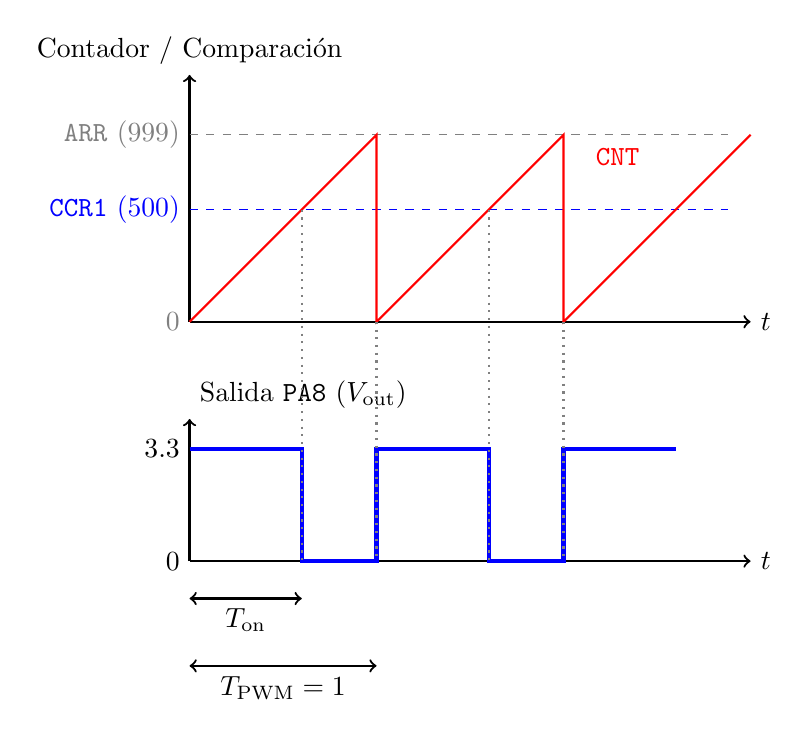
\begin{tikzpicture}[scale=0.95]
  % === SISTEMA SUPERIOR: CONTADOR CNT ===
  \draw[->, thick] (0,0) -- (7.5,0) node[right] {$t$};
  \draw[->, thick] (0,0) -- (0,3.3) node[above] {Contador / Comparación};

  % Niveles de referencia superior
  \draw[dashed, color=gray] (0,2.5) node[left] {\texttt{ARR} (999)} -- (7.2,2.5);
  \draw[dashed, color=blue] (0,1.5) node[left] {\texttt{CCR1} (500)} -- (7.2,1.5);
  \node[left, gray] at (0,0) {$0$};

  % Señal diente de sierra CNT
  \draw[thick, color=red] (0,0) -- (2.5,2.5) -- (2.5,0) -- (5,2.5) -- (5,0) -- (7.5,2.5);
  \node[red, right] at (5.3, 2.2) {\texttt{CNT}};

  % === SISTEMA INFERIOR: SALIDA PA8 ===
  \draw[->, thick] (0,-3.2) -- (7.5,-3.2) node[right] {$t$};
  \draw[->, thick] (0,-3.2) -- (0,-1.3) node[above right] {Salida \texttt{PA8} ($V_{\mathrm{out}}$)};

  % Formación de la onda cuadrada PWM en PA8
  \draw[ultra thick, color=blue] (0,-1.7) -- (1.5,-1.7) -- (1.5,-3.2) -- (2.5,-3.2) -- (2.5,-1.7) -- (4.0,-1.7) -- (4.0,-3.2) -- (5.0,-3.2) -- (5.0,-1.7) -- (6.5,-1.7);

  % Etiquetas de tensión en eje Y inferior
  \node[left] at (0,-1.7) {$\qty{3.3}{\V}$};
  \node[left] at (0,-3.2) {$\qty{0}{\V}$};

  % === LÍNEAS DE PROYECCIÓN VERTICAL ===
  \draw[dotted, thick, color=gray] (1.5,1.5) -- (1.5,-3.2);
  \draw[dotted, thick, color=gray] (2.5,0) -- (2.5,-3.2);
  \draw[dotted, thick, color=gray] (4.0,1.5) -- (4.0,-3.2);
  \draw[dotted, thick, color=gray] (5.0,0) -- (5.0,-3.2);

  % === COTAS TEMPORALES ===
  \draw[<->, thick] (0,-3.7) -- (1.5,-3.7) node[midway, below] {$T_{\mathrm{on}}$};
  \draw[<->, thick] (0,-4.6) -- (2.5,-4.6) node[midway, below] {$T_{\mathrm{PWM}} = \qty{1}{\ms}$};
\end{tikzpicture}

  \caption{Forma de onda PWM generada por comparación entre el contador \texttt{CNT} y el registro \texttt{CCR1}.}
  \label{fig.ej5:pwm_plot}
\end{figure}

\subsection{Efecto sobre la Tensión Promedio y el Brillo Percibido}
Al conmutar a alta frecuencia ($\qty{1}{\kHz}$), la respuesta óptica y eléctrica responde al valor medio de tensión ($V_{\mathrm{promedio}}$):

\begin{equation}
    V_{\mathrm{promedio}} = D \times V_{\mathrm{DD}} = \left( \frac{\text{CCR1}}{1000} \right) \times \qty{3.3}{\V}
    \label{eq.ej5:v_promedio}
\end{equation}

\begin{itemize}
    \item Para $\text{CCR1} = 0 \implies D = 0\% \implies V_{\mathrm{promedio}} = \qty{0}{\V}$ (LED apagado).
    \item Para $\text{CCR1} = 500 \implies D = 50\% \implies V_{\mathrm{promedio}} = \qty{1.65}{\V}$ (Brillo intermedio).
    \item Para $\text{CCR1} = 1000 \implies D = 100\% \implies V_{\mathrm{promedio}} = \qty{3.3}{\V}$ (Brillo máximo).
\end{itemize}

Al variar el valor de \lstinline{TIM1->CCR1} en el bucle principal de 0 a 1000, se modifica directamente el ancho del pulso activo
$T_{\mathrm{on}} = \text{CCR1} \times \qty{1}{\us}$, logrando el efecto visual continuo de incremento y decremento de intensidad.

\section{Código Fuente Final (\texttt{main.c})}
\label{sec.ej5:codigo_fuente}

En el listado~\ref{list.ej5:main} se adjunta el código fuente completo del programa en C desarrollado sobre CMSIS:

\lstinputlisting[language={C}, caption={Código fuente final del programa PWM y fading (\texttt{main.c}).}, label={list.ej5:main}]{sources/src/main.c}
